\documentclass{scrartcl}
\usepackage[utf8]{inputenc}
\usepackage[T1]{fontenc}
\usepackage[ngerman]{babel}
\usepackage{lmodern}
\usepackage{amssymb}
\usepackage{amsmath}
\usepackage{graphicx}
\usepackage{fancyhdr}
\pagestyle{fancy}
\usepackage{lastpage}
\usepackage{csquotes}
\usepackage{paralist}
\usepackage{longtable}
\usepackage{tabu}

% Makros
\newcommand*{\name}{Antigen}
\newcommand*{\tabref}[1]{Tab.~\ref{#1}}
\newcommand*{\figref}[1]{Abb.~\ref{#1}}
\newcommand*{\secref}[1]{Kap.~\ref{#1}}

% Layout
\setlength{\parindent}{0pt}
\setlength{\parskip}{.5em}
\setlength{\headheight}{30pt}

% Definition der Kopfzeile
\lhead{Game Design Document}
\chead{\name}
\rhead{Gruppe 2}
\lfoot{}
\cfoot{Seite \thepage{} von \pageref{LastPage}}
\rfoot{}

\begin{document}

% Title page
\title{\name\\Game Design Document\thanks{Gruppe 2, Sabine Rogg}}
\author{Layla Franke \and Thomas Lang \and Jannis Limperg \and Daniel Tischner
        \and Silas Zimmermann}
\date{\today}
\maketitle
\newpage

\section{Spielkonzept}
\label{sec:spielkonzept}
\subsection{Zusammenfassung}
%Hier ist ein kurzer einleitender Text evtl. in Verbindung mit einem Bild gefragt. Ziel ist es, das zu erstellende Spiel in kurzen Sätzen zu erklären und die Grundidee zu erläutern. Für die Zusammenfassung kann man sich an den "Klappentexten" auf der Rückseite von Spieleverpackungen orientieren. Der Text darf als einziger im GDD auch reißerisch und dramatisch sein (abgesehen vom Screenplay).

Eine Geschichte, die uns alle betrifft: die Realität. Tag für Tag wehrt sich der
menschliche Körper gegen alle Arten von Angriffen. Dabei sind häufig diejenigen
Bedrohungen am gefährlichsten, die man nicht sehen kann. Trotzdem gibt
es immer wieder Menschen, die diesen gefahrlos begegnen können, während andere
an ihnen zugrunde gehen. Doch wie geht das alles vor sich? \enquote{\name} ist ein
2D-Echtzeitstrategiespiel, das bewusst an die Realität angelehnt ist. Der
Spieler hat die Möglichkeit, sich verschiedener Abwehrmechanismen zur Bekämpfung
der drohenden Krankheiten zu bedienen. Werden diese geschickt kombiniert, kann
es ihm gelingen, die angreifenden Viren und Bakterien in die Flucht zu
schlagen.

\subsection{Alleinstellungsmerkmal}
%Was hebt dieses Spiel von der Masse ab? Wodurch versucht man, den Spieler (und den Kunden) zu begeistern? Das Alleinstellungsmerkmal ist das Merkmal des Spiels, welches es einzigartig macht. Ein Alleinstellungsmerkmal kann sowohl ein Feature, als auch ein gesamtes Konzept des Spiels sein.

Durch sein flexibles Mutationssystem erlaubt Antigen es dem Spieler, Zellen
nach Belieben anzupassen. Mutationen können alle Eigenschaften seiner Zellen,
von Lebenspunkten über Virenresistenz bis zur Sichtweite, verändern, sodass am
Ende eine für die Bekämpfung des Gegners maßgeschneiderte Einheit steht. Doch
das gleiche System steht auch der KI zur Verfügung, die versuchen wird, die
Anpassungen des Spielers zu unterlaufen. Außerdem gehen die meisten
Verbesserungen einer Eigenschaft mit Verschlechterungen in anderen Bereichen
einher, sodass die spezialisiertesten Zellen auch am anfälligsten für Konter
sind.


\section{Benutzeroberfläche}
\label{sec:benutzeroberflaeche}
\subsection{Spielwelt und Kamera}

Die Spielwelt (Illustration s. \figref{fig:hud}) besteht aus einem System von
Blutbahnen, dem Blutkreislauf, in dem sich die Zellen des Spielers und die
gegnerischen Viren und Bakterien aufhalten.

Die Kamera zeigt stets einen Ausschnitt des Blutkreislaufs, wobei die Größe
des dargestellten Ausschnitts und seine Position vom Spieler wählbar sind.

Gegnerische Einheiten und rote Blutkörperchen sind für den Spieler nur
sichtbar, sofern sie sich im Sichtkreis einer seiner Einheiten befinden. Die
Teile der Spielwelt, die nicht im Sichtkreis einer solchen Einheit liegen,
werden abgedunkelt dargestellt (\enquote*{Fog of War}).

\begin{figure}
  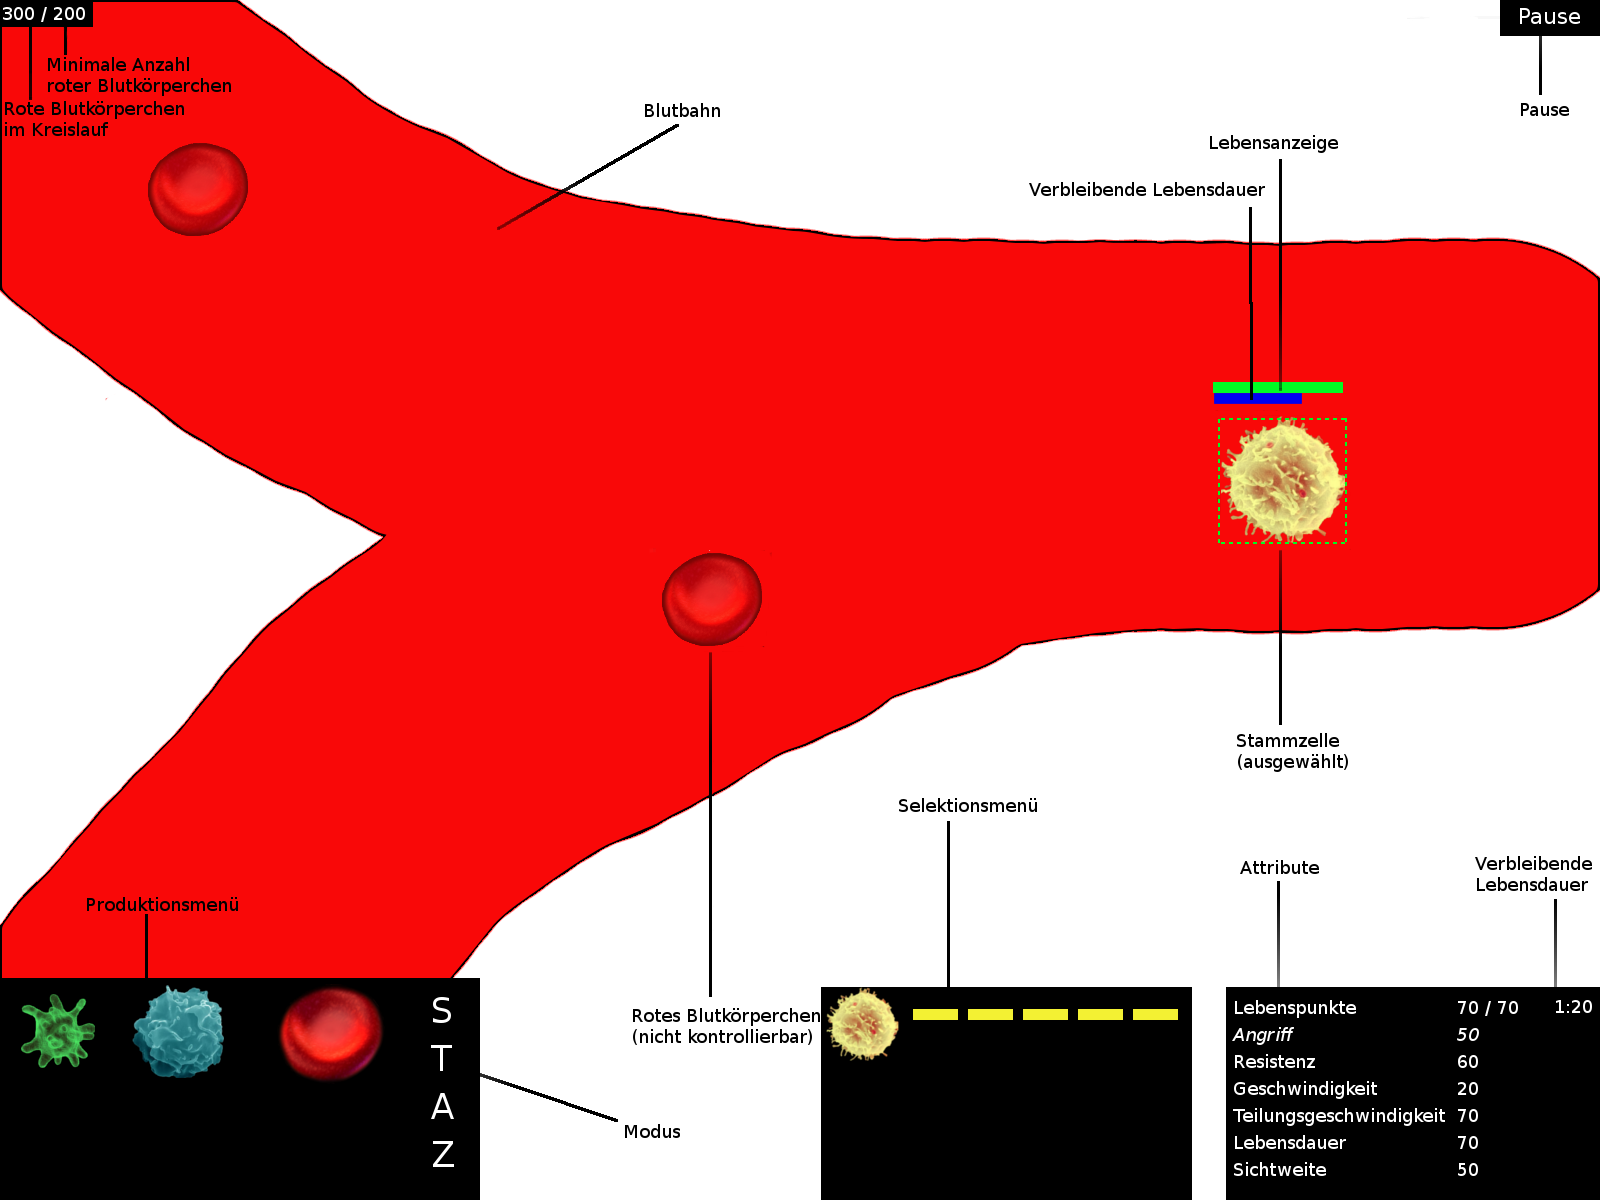
\includegraphics[width=\textwidth]{img_ui/hud}
  \caption{Spielwelt und Heads Up Display (Konzept)}
  \label{fig:hud}
\end{figure}

\subsection{Kontrollschema}

\name{} wird vorwiegend mit der Maus gesteuert: Alle Aktionen können allein mit
der Maus vorgenommen werden, aber für manche sind auch Tastenkombinationen
definiert. Im folgenden Überblick über das Kontrollschema ist jeweils die
Standardtastenbelegung angegeben.

Das Produktionsmenü, die Modusauswahl und der Link zum Pausemenü sind
Elemente des Heads Up Displays, die in \figref{fig:hud} illustriert sind.

\newcommand*{\shortcut}[1]{\textbf{#1}}

\begin{description}
  \item[Cursorbewegung] Wird der Cursor an den Rand des Spielfensters
    geführt, so wird die Karte in die entsprechende Richtung bewegt, sofern
    sie in dieser Richtung nicht bereits den Rand der Karte erreicht hat.
  \item[Mausrad] Ein Drehen des Mausrads nach vorn zoomt in das Spiel herein;
    ein Drehen nach hinten aus dem Spiel heraus.
  \item[Linke Maustaste] Ein Klick auf eine auswählbare Einheit wählt diese
    aus. Durch Klicken und Halten kann ein Rechteck aufgezogen werden, mit
    dem alle auswählbaren Einheiten in einem Bereich ausgewählt werden.
  \item[Rechte Maustaste]
    Die Belegung der rechten Maustaste variiert abhängig von der ausgewählten
    Einheit und dem Ziel des Klicks.
    \begin{itemize}
      \item Ausgewählte bewegbare Einheit, Klick auf den Boden: Die ausgewählte
        Einheit bewegt sich zum angegebenen Punkt oder, wenn das nicht
        möglich ist, zu einem möglichst nahen erreichbaren Punkt.
      \item Ausgewählte angreifende Einheit, Klick auf eine gegnerische Einheit:
        Sofern die ausgewählte Einheit die gegnerische Einheit angreifen kann,
        bewegt jene sich zu dieser und attackiert sie.
      \item Ausgewählte antigenverarbeitende Einheit, Klick auf Riesenfresszelle:
        Sofern die Riesenfresszelle ein Antigen aufgenommen hat, bewegt sich
        die ausgewählte Einheit zu ihr und übernimmt das Antigen.
      \item Ausgewählte Riesenfresszelle mit Antigen, Klick auf
        antigenverarbeitende Zelle: Die Riesenfresszelle bewegt sich zur
        angeklickten Einheit und übergibt ihr das Antigen.
    \end{itemize}
  \item[Überblick] (\shortcut{Leertaste}) Verändert den Kameraausschnitt so,
    dass die Spielwelt vollständig sichtbar ist.
  \item[Produktionsmenü] Produziert bei ausgewählter Stammzelle eine
    B-Zelle (\shortcut{B}), T-Zelle (\shortcut{T}), Riesenfresszelle
    (\shortcut{F}) oder ein Rotes Blutkörperchen (\shortcut{R}). Bei
    ausgewählter B-Zelle kann ein Antikörper (\shortcut{A}) produziert werden.
    Siehe auch \secref{sec:zellen}.
  \item[Modusauswahl] Wählt bei ausgewählter eigener Einheit einen der vier
    Zellmodi (siehe \secref{sec:modi}) aus: Stellung halten (\shortcut{S}),
    Treiben lassen (\shortcut{L}), Angriff (\shortcut{P}) oder Zellteilung
    (\shortcut{Z}).
  \item[Pause] Pausiert das Spiel (\shortcut{Esc}).
\end{description}

\subsection{Heads Up Display}

Außer den im letzten Abschnitt erwähnten interaktiven Elementen des HUD
(\figref{fig:hud}) enthält dieses noch die folgenden informativen Elemente:

\begin{description}
  \item[Zähler für Rote Blutkörperchen:] Zeigt die aktuelle Anzahl Roter
    Blutkörperchen im Blutkreislauf und die Minimalanzahl, bei deren
    Unterschreitung das Spiel verloren ist.
  \item[Lebensanzeigen:] Grafische Repräsentation der aktuellen Lebenspunkte
    jeder ausgewählten Einheit.
  \item[Attributanzeige:] Aktuelle Werte der Eigenschaften
    (s.~\tabref{tab:eigenschaften}) der ausgewählten Einheit.
  \item[Verbleibende Lebensdauer:] Anzeige der verbleibenden Zeit, nach der die
    ausgewählte Einheit \enquote*{natürlich} stirbt.
  \item[Selektionsmenü:] Liste aller selektierten Einheiten mit einer
    Übersicht über ihre Attributwerte.
\end{description}

\subsection{Menüstruktur}

\subsubsection{Hauptmenü}
\label{menu:hauptmenu}

\begin{description}
  \item[Neues Spiel] (\ref{menu:neues_spiel})
  \item[Laden] (\ref{menu:laden})
  \item[Optionen] (\ref{menu:optionen})
  \item[Achievements] (\ref{menu:achievements})
  \item[Ende] Beendet das Programm.
\end{description}

\subsubsection{Pause}
\label{menu:pause}

\begin{description}
  \item[Fortsetzen] Kehrt zum Spiel zurück.
  \item[Speichern] (\ref{menu:speichern})
  \item[Laden] (\ref{menu:laden})
  \item[Optionen] (\ref{menu:optionen})
  \item[Statistiken] (\ref{menu:statistiken})
  \item[Achievements] (\ref{menu:achievements})
  \item[Hauptmenü] Beendet das aktuelle Spiel, ohne zu speichern, und kehrt
    zum Hauptmenü zurück.
  \item[Ende] Beendet das Programm.
\end{description}

\subsubsection{Neues Spiel}
\label{menu:neues_spiel}

Auswahl der Karte und des Schwierigkeitsgrads für ein neues Spiel.

Der Schwierigkeitsgrad kann die Werte Leicht/Mittel/Schwer annehmen. Ein
leichterer Schwierigkeitsgrad erhöht die Werte einiger Einheiten des
Spielers und senkt die einiger Einheiten der KI. Er modifiziert \textbf{optional}
auch das Verhalten der KI, wobei ein leichterer Schwierigkeitsgrad dazu führt,
dass die KI mehr taktische Fehler begeht.

\subsubsection{Speichern}
\label{menu:speichern}

Zeigt eine Liste mit vorhandenen Spielständen. Das aktuelle Spiel kann entweder
einen dieser Spielstände überschreiben oder als neuer Spielstand gespeichert
werden. Für Spielstände können Namen vergeben werden, außerdem sind sie mit
einer eindeutigen Nummer gekennzeichnet.

\subsubsection{Laden}
\label{menu:laden}

Zeigt eine Liste mit vorhandenen Spielständen, von denen einer ausgewählt
werden kann.

\subsubsection{Optionen}
\label{menu:optionen}

Ermöglicht die Anpassung der folgenden Optionen (ggf. mit eigenen Untermenüs):

\begin{description}
  \item[Kamerageschwindigkeit:] 0,5x bis 2x. Multipliziert die Geschwindigkeit
    der Kamerabewegung bei Veränderung des Kameraausschnitts mit dem
    entsprechenden Faktor.
  \item[Auflösung:] Modifiziert die Auflösung der grafischen Darstellung des
    Spiels. Der Spieler kann jede Auflösung wählen, die sein Anzeigegerät
    unterstützt. Die Spielbarkeit des Spiels wird allerdings nur für
    Auflösungen zwischen 1024x798 und 1920x1080 Pixeln garantiert.
  \item[Vollbild:] Stellt das Spiel im Vollbildmodus dar. Ist diese Option
    nicht ausgewählt, so wird das Spiel im Fenstermodus dargestellt.
  \item[Audio:] Modifiziert die Lautstärke der Spielsounds. Separate Optionen
    für Master-, Musik- und Effektlautstärke.
  \item[Tastenbelegung:] Assoziiert Aktionen mit Tasten.
\end{description}

\subsubsection{Statistiken}
\label{menu:statistiken}

Zeigt Statistiken (s.~\secref{sec:statistiken}) für das gerade laufende Spiel
an.

\subsubsection{Achievements}
\label{menu:achievements}

Zeigt die bislang über alle Spiele errungenen Achievements
(s.~\secref{sec:achievements}) an.


\section{Spiellogik}
\label{sec:spiellogik}

\subsection{Grundlegende Spielmechaniken}
\label{sec:spielmechaniken}
Viele Mechaniken von \name{} sind denen in anderen Echtzeitstrategiespielen
ähnlich. Sie werden in den folgenden Abschnitten detailliert beschrieben. Dieser
Abschnitt soll dagegen einen Überblick über die ungewöhnlicheren Spielmechaniken
geben.

\subsubsection{Zellteilung und Mutation}

Neue Zellen werden primär durch Zellteilung produziert. Dabei können die
meisten Zellen sich nur reproduzieren, also Klone von sich selbst erschaffen.
Manche Zellen haben aber auch die Fähigkeit, andere Zelltypen gezielt
herzustellen.

Bei der Zellteilung werden die Eigenschaften der sich teilenden Zelle im
Regelfall unverändert auf ihren Klon übertragen. Mit relativ geringer
Wahrscheinlichkeit tritt allerdings eine Mutation auf, d.h. die Werte des
Klons weichen positiv oder negativ von denen des Originals ab.

In der Spielwelt gibt es bestimmte Bereiche -- Mutationsfelder --, in denen
Mutationen mit deutlich größerer Wahrscheinlichkeit auftreten. Zusätzlich
verändern verschiedene Mutationsfelder verschiedene Eigenschaften der Zellen
unterschiedlich stark.

Die durch Mutationsfelder verursachten Werteänderungen streben einem
Normalniveau entgegen, sodass eine Zelle mit insgesamt besseren Werten
wahrscheinlicher verschlechtert als weiter verbessert wird.

\subsubsection{Antigene}

Jedes Bakterium und jedes Virus trägt eines von mehreren Antigenen in sich.
Diese Antigene können durch Riesenfresszellen extrahiert und anschließend
zur Produktion spezialisierter Abwehrzellen verwendet werden.

Bei der Produktion neuer Bakterien und Viren kann mit sehr geringer
Wahrscheinlichkeit das Antigen mutieren, sodass die neu entstandene Zelle
ein anderes Antigen als die produzierende Zelle trägt. In Mutationsfeldern
ist die Wahrscheinlichkeit hierfür wiederum deutlich erhöht.

\subsubsection{Infektion}

Viren können Zellen des Spielers infizieren, sofern ihre Infektionsstärke die
Virenresistenz der zu infizierenden Zelle übersteigt. Mit der Infektion
verliert der Spieler die Kontrolle über die infizierte Zelle und sie beginnt,
weitere Viren zu produzieren.

Wie bei der Zellteilung werden auch bei der Produktion von Viren durch
infizierte Zellen die Eigenschaften des Virus, das die Zelle befallen hat,
im Regelfall unverändert vererbt, können sich aber durch Mutation ändern.


\subsection{Spielobjekte}
\label{sec:spielobjekte}
\subsubsection{Zellen}
\label{sec:zellen}

Zellen sind dynamische Spielobjekte, die entweder vom Spieler oder von der KI
kontrolliert werden oder sich neutral verhalten. Sie haben eine oder mehr
der Eigenschaften aus \tabref{tab:eigenschaften}.

Die Eigenschaften unterteilen sich in persistente, die sich während des
Lebenszyklus einer Zelle nicht ändern, und nicht persistente, die sich
nach der Entstehung einer Zelle noch ändern können. Alle persistenten
Eigenschaften können sich aber bei der Zellteilung oder der Produktion von Viren
durch Mutation ändern.

\begin{table}
  \begin{tabu} to \linewidth {|l|X|}
    \hline
    Eigenschaft &
      Beschreibung\\\hline

    Maximale Lebenspunkte &
      Maximale Lebenspunkte einer Zelle. Wertebereich 1 (schwach) bis 100
      (stark).\\\hline

    Aktuelle Lebenspunkte &
      Lebenspunkte einer Zelle von 0 (tot) bis zum durch die Eigenschaft
      Maximale Lebenspunkte vorgegebenen Maximalwert. Direkt nach ihrer
      Entstehung entsprechen die aktuellen Lebenspunkte einer Zelle ihren
      maximalen Lebenspunkten. Durch Angriffe gegnerischer Zellen können
      die aktuellen Lebenspunkte reduziert werden. Erreichen die aktuellen
      Lebenspunkte den Wert 0, stirbt die Zelle. Diese Eigenschaft ist
      nicht persistent.\\\hline

    Initiale Lebensdauer &
      Zeitspanne, nach der eine Zelle unabhängig von ihren aktuellen
      Lebenspunkten \enquote*{natürlich} stirbt, in Sekunden ab ihrer
      Entstehung.\\\hline

    Verbleibende Lebensdauer &
      Zeitspanne, nach der eine Zelle unabhängig von ihren aktuellen
      Lebenspunkten \enquote*{natürlich} stirbt, in Sekunden ab dem aktuellen
      Zeitpunkt. Verringert sich jede Sekunde um eins. Bei Entstehung der
      Zelle entspricht dieser Wert der Initialen Lebensdauer. Diese
      Eigenschaft ist nicht persistent.\\\hline

    Angriffsstärke &
      Anzahl der Lebenspunkte pro Sekunde, die die Zelle einer gegnerischen
      Zelle beim Angriff abzieht.\\\hline

    Geschwindigkeit &
      Bewegungsgeschwindigkeit einer Zelle. Wertebereich 1 (langsam) bis 100
      (schnell).\\\hline

    Zellteilungsgeschwindigkeit &
      Dauer einer Zellteilung in Sekunden, von ihrer Initiation bis zum
      Entstehen der neuen Zelle.\\\hline

    Sichtweite &
      Sichtweite einer Zelle. Wertebereich 1 (kurz) bis (100 lang).\\\hline

    Antigen &
      Spezielle Eigenschaft von Viren, Bakterien, B-, T-, und Riesenfresszellen
      sowie Antikörpern. Siehe \secref{sec:spielmechaniken} und
      \secref{sec:optionen_aktionen} für Details zu den assoziierten
      Spielmechaniken.\\\hline

    Virenresistenz &
      Resistenz einer Zelle gegen Virenangriffe. Übersteigt die
      Infektionsstärke eines angreifenden Virus die Virenresistenz der
      angegriffenen Zelle, so wird die Zelle vom Virus übernommen. Wertebereich
      1 (schwach) bis 100 (stark).\\\hline

    Infektionsstärke &
      Angriffsstärke eines Virus. Übersteigt dieser Wert die Virenresistenz
      einer gegnerischen Zelle, so kann die Zelle vom Virus übernommen werden.
      Wertebereich 1 (schwach) bis 100 (stark).\\\hline

  \end{tabu}
  \caption{Eigenschaften. Wo nicht anders gekennzeichnet, sind die
  Eigenschaften persistent.}
  \label{tab:eigenschaften}
\end{table}

Im Folgenden werden alle Zellen des Spiels aufgeführt. Die angegebenen
Eigenschaftswerte für Lebensdauer und Zellteilungsgeschwindigkeit geben nur
näherungsweise die Verhältnisse zwischen verschiedenen Einheiten an, nicht aber
die absoluten Werte in Sekunden.

% Params:
%    1 Name
%    2 Dateiname des Bildes
%    3 kontrolliert durch
%    4 Beschreibung
%    5 Max. Lebenspunkte
%    6 Initiale Lebensdauer
%    7 Angriffsstärke
%    8 Geschwindigkeit
%    9 Zellteilungsgeschwindigkeit
%   10 Sichtweite
%   11 Virenresistenz
%   12 Infektionsstärke
%   13 attackiert
%   14 attackiert von
%   15 produziert von
%   16 produziert
\newcommand\cellentry[9]{%
  \minisec{#1}%
  #4%

  %\multicolumn{2}{|c|}{#1}\\%
  %\multicolumn{2}{|c|}{\includegraphics[width=2cm]{img_objekte/#2}}\\%
  \begin{tabular} {|l|p{9cm}|}%
    \hline%
    kontrolliert durch          & #3\\\hline%
    Maximale Lebenspunkte       & #5\\\hline%
    Initiale Lebensdauer        & #6\\\hline%
    Angriffsstärke              & #7\\\hline%
    Geschwindigkeit             & #8\\\hline%
    Zellteilungsgeschwindigkeit & #9\\\hline%
}%

\newcommand\cellentryctd[7]{%
    Sichtweite                  & #1\\\hline%
    Virenresistenz              & #2\\\hline%
    Infektionsstärke            & #3\\\hline%
    attackiert                  & #4\\\hline%
    attackiert von              & #5\\\hline%
    produziert von              & #6\\\hline%
    produziert                  & #7\\\hline%
  \end{tabular}%
}

\cellentry
  {Stammzelle}
  {stemcellorig}
  {Spieler}
  {Produziert durch Zellteilung alle vom Spieler kontrollierten
   Zellen (außer Antikörpern) sowie rote Blutkörperchen.
   Die Zellteilung einer Stammzelle dauert
   wesentlich kürzer als die anderer Einheiten. Stammzellen können nicht
   angreifen.
  }
  {70} % Max. Lebenspunkte
  {70} % Initiale Lebensdauer
  {--} % Angriffsstärke
  {20} % Geschwindigkeit
  {70} % Zellteilungsgeschwindigkeit
\cellentryctd
  {50} % Sichtweite
  {60} % Virenresistenz
  {--} % Infektionsstärke
  {--} % attackiert
  {Bakterium, Virus} % attackiert von
  {Stammzelle} % produziert von
  {Stamm-, B-, T-, Riesenfresszelle; rote Blutkörperchen} % produziert

\cellentry
  {B-Zelle}
  {bcellorig}
  {Spieler}
  {B-Zellen können Antikörper produzieren, sofern sie ein Antigen besitzen. Das
   Antigen kann von einer Riesenfresszelle, die zuvor eine gegnerische Zelle
   getötet hat, übernommen werden. Es wird an die produzierten Antikörper
   sowie an durch Zellteilung produzierte B-Zellen weitergegeben. B-Zellen
   können nicht angreifen.
  }
  {30} % Max. Lebenspunkte
  {30} % Initiale Lebensdauer
  {--} % Angriffsstärke
  {40} % Geschwindigkeit
  {20} % Zellteilungsgeschwindigkeit
\cellentryctd
  {50} % Sichtweite
  {30} % Virenresistenz
  {--} % Infektionsstärke
  {--} % attackiert
  {Bakterium, Virus} % attackiert von
  {Stammzelle, B-Zelle} % produziert von
  {Antikörper, B-Zelle} % produziert

\cellentry
  {T-Zelle}
  {tcellorig}
  {Spieler}
  {Spezialisierte Angriffseinheit gegen infizierte Zellen. Kann ausschließlich
   infizierte Zellen, deren Antigen sie besitzt, attackieren. Erhält ihr Antigen
   von einer Riesenfresszelle, nachdem diese eine gegnerische Zelle getötet
   und ihr Antigen extrahiert haben. Gibt bei der Zellteilung ihr Antigen
   an die neu entstandene Zelle ab.
  }
  {60} % Max. Lebenspunkte
  {40} % Initiale Lebensdauer
  {30 (+ 30 mit Antigenbonus)} % Angriffsstärke
  {50} % Geschwindigkeit
  {20} % Zellteilungsgeschwindigkeit
\cellentryctd
  {50} % Sichtweite
  {50} % Virenresistenz
  {--} % Infektionsstärke
  {Infizierte Zelle} % attackiert
  {Bakterium, Virus} % attackiert von
  {Stammzelle, T-Zelle} % produziert von
  {T-Zelle} % produziert

\cellentry
  {Riesenfresszelle}
  {fresszelleorig}
  {Spieler}
  {Angriffseinheit, die Bakterien und Viren, aber keine infizierten Zellen
   attackieren kann. Kann keine Zellteilung durchführen. Tötet eine
   Riesenfresszelle eine gegnerische Einheit, so nimmt sie deren Antigen
   auf und kann dieses an eine T- oder B-Zelle weitergeben.
  }
  {50} % Max. Lebenspunkte
  {30} % Initiale Lebensdauer
  {40} % Angriffsstärke
  {50} % Geschwindigkeit
  {--} % Zellteilungsgeschwindigkeit
\cellentryctd
  {50} % Sichtweite
  {30} % Virenresistenz
  {--} % Infektionsstärke
  {Bakterium, Virus} % attackiert
  {Bakterium, Virus} % attackiert von
  {Stammzelle} % produziert von
  {--} % produziert

\cellentry
  {Antikörper}
  {antikoerperorig}
  {Spieler}
  {Angriffseinheit, die gegnerische Zellen befallen kann. Durch den Befall
   werden die Werte der persistenten Eigenschaften der befallenen Zelle
   dauerhaft verringert (\enquote*{Debuff}) und der befallende Antikörper
   vernichtet. Antikörper übernehmen das Antigen der sie produzierenden B-Zelle
   und können nur Zellen mit diesem Antigen angreifen. Antikörper können keine
   Zellteilung durchführen.
  }
  {30} % Max. Lebenspunkte
  {40} % Initiale Lebensdauer
  {--} % Angriffsstärke
  {70} % Geschwindigkeit
  {--} % Zellteilungsgeschwindigkeit
\cellentryctd
  {50} % Sichtweite
  {20} % Virenresistenz
  {--} % Infektionsstärke
  {Bakterium/Virus mit dem Antigen des Antikörpers} % attackiert
  {Bakterium, Virus} % attackiert von
  {B-Zelle mit Antigen} % produziert von
  {--} % produziert

\cellentry
  {Rotes Blutkörperchen}
  {redbloodcella}
  {neutral}
  {Neutrale Zelle, die vom Spieler produziert und von Bakterien und Viren
   angegriffen werden kann. Wird nicht vom Spieler kontrolliert und bewegt
   sich passiv mit dem Blutstrom. Kann keine Zellteilung durchführen und
   gewährt dem Spieler keine Sicht in seinem Umkreis.
  }
  {30} % Max. Lebenspunkte
  {40} % Initiale Lebensdauer
  {--} % Angriffsstärke
  {50} % Geschwindigkeit
  {--} % Zellteilungsgeschwindigkeit
\cellentryctd
  {--} % Sichtweite
  {20} % Virenresistenz
  {--} % Infektionsstärke
  {--} % attackiert
  {Bakterium, Virus} % attackiert von
  {Stammzelle} % produziert von
  {--} % produziert

\cellentry
  {Bakterium}
  {bakteriumorig}
  {KI}
  {Angriffseinheit der gegnerischen KI. Besitzt die Eigenschaft Antigen, die
   bei der Zellteilung im Regelfall an das produzierte Bakterium vererbt
   wird. Es besteht allerdings eine geringe Wahrscheinlichkeit, dass das
   produzierte Bakterium zufällig ein anderes Antigen als das produzierende
   erhält.
  }
  {50} % Max. Lebenspunkte
  {30} % Initiale Lebensdauer
  {40} % Angriffsstärke
  {50} % Geschwindigkeit
  {30} % Zellteilungsgeschwindigkeit
\cellentryctd
  {50} % Sichtweite
  {--} % Virenresistenz
  {--} % Infektionsstärke
  {Stammzelle, Riesenfresszelle, T-Zelle, B-Zelle, Antikörper, rotes Blutkörperchen} % attackiert
  {Riesenfresszelle, Antikörper} % attackiert von
  {Bakterium} % produziert von
  {Bakterium} % produziert

\cellentry
  {Virus}
  {virusaorig}
  {KI}
  {Angriffseinheit der KI. Kann die Lebenspunkte gegnerischer Zellen nicht
   reduzieren, aber sie infizieren. Wird eine Einheit infiziert, so
   transformiert sie sich in eine infizierte Zelle, die nicht mehr vom
   Spieler kontrolliert wird. Das infizierende Virus wird dabei vernichtet.
   Jedes Virus besitzt ein Antigen, das bei
   der Infektion einer Zelle an die dadurch entstehende infizierte Zelle
   weitergegeben wird. Viren können keine Zellteilung durchführen. Die
   Eigenschaft \emph{Zellteilungsgeschwindigkeit} ist stattdessen dafür
   maßgeblich, wie schnell eine durch ein Virus infizierte Zelle neue
   Viren produziert.
  }
  {40} % Max. Lebenspunkte
  {40} % Initiale Lebensdauer
  {--} % Angriffsstärke
  {40} % Geschwindigkeit
  {40} % Zellteilungsgeschwindigkeit
\cellentryctd
  {50} % Sichtweite
  {--} % Virenresistenz
  {30} % Infektionsstärke
  {Stammzelle, Riesenfresszelle, T-Zelle, B-Zelle, Antikörper, rotes Blutkörperchen} % attackiert
  {Riesenfresszelle, Antikörper} % attackiert von
  {infizierte Zelle} % produziert von
  {infizierte Zelle (durch Infektion)} % produziert

\cellentry
  {Infizierte Zelle}
  {infectedcell}
  {KI}
  {Produktionseinheit der KI. Entsteht durch Infektion einer Zelle des
   Spielers oder eines roten Blutkörperchens. Erbt die Antigeneigenschaft
   von dem infizierenden Virus und alle anderen Eigenschaften von der
   Zelle, die von dem Virus infiziert wurde. Produziert kontinuierlich Viren,
   auf die das Antigen der infizierten Zelle im Regelfall vererbt wird. Mit
   geringer Wahrscheinlichkeit werden allerdings auch Viren mit einem
   zufälligen anderen Antigen produziert. Infizierte Zellen können nicht
   angreifen.
  }
  {geerbt bei Infektion} % Max. Lebenspunkte
  {geerbt bei Infektion} % Initiale Lebensdauer
  {--} % Angriffsstärke
  {geerbt bei Infektion} % Geschwindigkeit
  {geerbt von infizierendem Virus} % Zellteilungsgeschwindigkeit
\cellentryctd
  {geerbt bei Infektion}
  {--} % Virenresistenz
  {--} % Infektionsstärke
  {--} % attackiert
  {T-Zelle} % attackiert von
  {Virus (durch Infektion)} % produziert von
  {Virus} % produziert

\subsubsection{Sonstige Objekte}

\minisec{Blutbahn}

\begin{figure}
  \begin{center}
  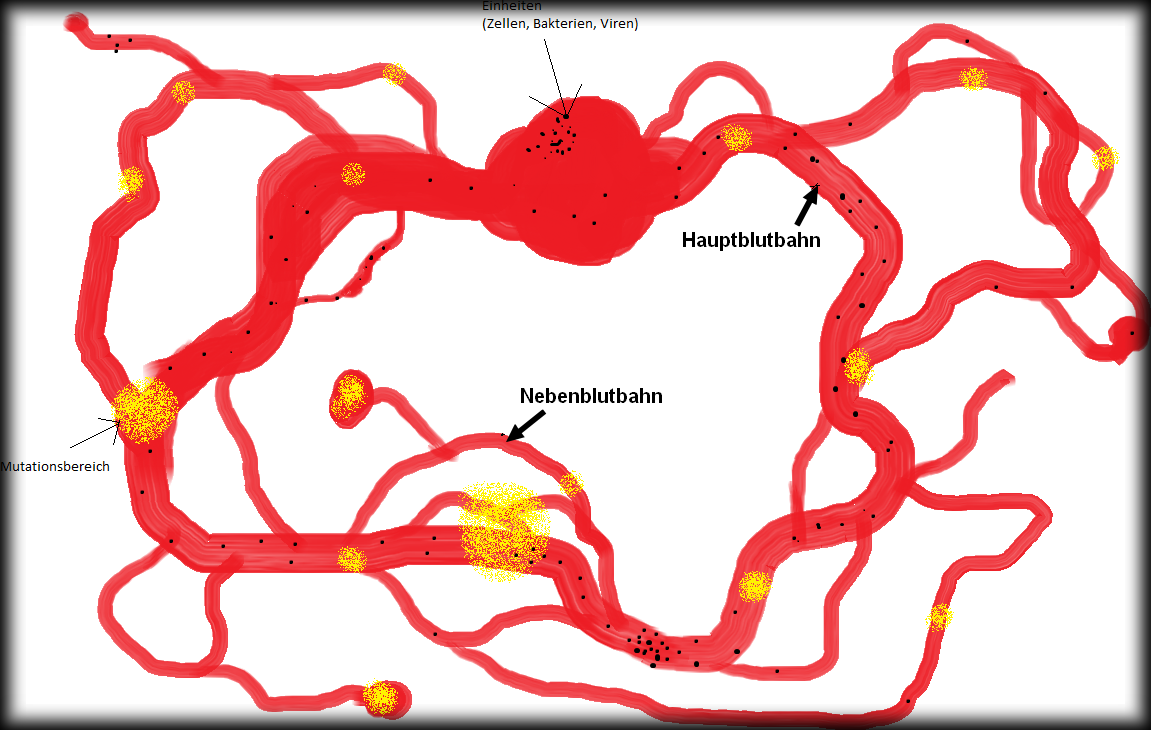
\includegraphics[width=10cm]{./img_objekte/blutbahn.png}\\
  \end{center}

  \caption{Blutbahnen}
  \label{fig:blutbahnen}
\end{figure}

Blutbahnen (Illustration s. \figref{fig:blutbahnen}) sind die begehbaren
Bereiche der Spielkarte. In Blutbahnen herrscht ein gerichteter Blutfluss, mit
dem sich Zellen treiben lassen können. (Siehe \secref{sec:aktionen}.)

\minisec{Mutationsfeld}

\begin{figure}
  \begin{center}
    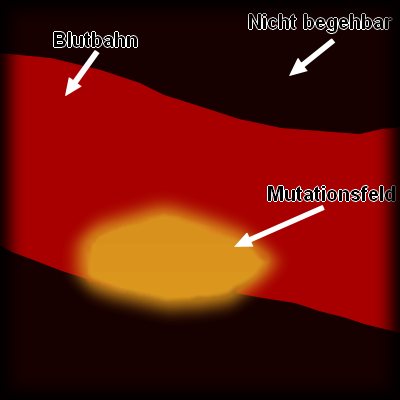
\includegraphics[width=5cm]{./img_objekte/mutationsfeld.png}\\
  \end{center}

  \caption{Mutationsfeld}
  \label{fig:mutationsfeld}
\end{figure}

Mutationsfelder (Illustration s. \figref{fig:mutationsfeld}) sind zufällig
auf Blutbahnen verteilte, persistente, begehbare Bereiche. Teilt sich eine Zelle,
während sie auf einem solchen Feld steht, so mutiert sie mit hoher
Wahrscheinlichkeit.

Verschiedene Mutationsfelder priorisieren verschiedene Eigenschaften
(beispielsweise Angriffsstärke), die wahrscheinlicher als andere Eigenschaften
bei der Mutation geändert werden. Jedes Mutationsfeld bietet jedoch eine
deutlich erhöhte Wahrscheinlichkeit der Änderung des Antigens von Viren
und Bakterien.


\subsection{Optionen und Aktionen}
\label{sec:optionen_aktionen}
\subsubsection{Zellmodi}
\label{sec:modi}

Zellen befinden sich zu jedem Zeitpunkt in einem von vier Modi und verhalten
sich ohne weitere Interaktion des Nutzers ihrem aktuellen Modus entsprechend.

\begin{description}
  \item[Angriff] Die Zelle greift die erste gegnerische Zelle, die ihren
    Sichtradius betritt, an und verfolgt sie, bis die gegnerische Zelle tot
    oder außer Sichtweite ist. Kommen mehrere Zellen für die Auswahl des
    Ziels infrage, so wird die räumlich nächste gewählt.
  \item[Stellung halten] Die Zelle bewegt sich nicht und reagiert nicht
    auf gegnerische Zellen in ihrer Sichtweite, außer wenn diese in
    Angriffsreichweite sind. In diesem Fall attackiert die Zelle die
    gegnerische Zelle, bis jene tot oder nicht mehr in Angriffsreichweite
    ist.
  \item[Treiben lassen] Die Zelle bewegt sich mit dem Blutfluss und
    verhält sich dabei passiv, reagiert also nicht auf Zellen in ihrer
    Umgebung.
  \item[Zellteilung] Die Zelle teilt sich und produziert kontinuierlich,
    in einem von ihrer Zellteilungsgeschwindigkeit bestimmten Intervall,
    neue Zellen. Dabei verhält sie sich passiv, reagiert also nicht auf
    Zellen in ihrer Umgebung, und bewegt sich nicht.
\end{description}

\subsubsection{Aktionen}
\label{sec:aktionen}

Im Folgenden werden alle Aktionen, mit denen der Spieler oder die KI den
Zustand des Spiels beeinflussen können, dargestellt.

\newcounter{usecasect}

\newcommand*{\oder}{\textbf{oder} }
\newcommand*{\actionentry}[5]{%
  \stepcounter{usecasect}
  \minisec{\theusecasect . #1}%
%
  \begin{tabular}{|l|p{9cm}|}%
    \hline%
    Akteur & #2\\%
    Startbedingung & #3\\%
    Schlussbedingung & #4\\%
    \hline%
  \end{tabular}%
%
  #5%
}

\actionentry
{Eine Zelle auswählen}
{Spieler}
{--}
{Die Einheit ist ausgewählt. Alle anderen Einheiten sind abgewählt.}
{
  \begin{compactenum}
    \item Der Spieler linksklickt auf eine auswählbare Einheit.
    \item Die Einheit wird ausgewählt.
  \end{compactenum}
}

\actionentry
{Mehrere Zellen auswählen}
{Spieler}
{--}
{
  Alle auswählbaren Einheiten im Rechteck sind ausgewählt. Alle anderen
  Einheiten sind abgewählt.
}
{
  \begin{compactenum}
    \item Der Spieler zieht ein Auswahlrechteck auf, in dem sich mindestens
      eine auswählbare Einheit befindet.
    \item Die auswählbaren Einheiten im Auswahlrechteck werden ausgewählt.
  \end{compactenum}
}

\actionentry
{Einheiten zu erreichbarem Punkt bewegen}
{Spieler oder KI}
{Es sind kontrollierbare Einheiten ausgewählt.}
{Die ausgewählten Einheiten befinden sich am Zielpunkt.}
{
  \begin{compactenum}
    \item Der Akteur klickt mit der rechten Maustaste auf einen begehbaren
      Punkt in der Welt.
    \item Ausgewählte Einheiten, die sich vorher im Treiben- oder
      Zellteilungsmodus befanden, wechseln in den Angriffsmodus.
    \item Die ausgewählten Einheiten bewegen sich ausgehend von ihrer
      Position auf dem kürzesten Weg auf den Punkt zu.
    \item Die ausgewählten Einheiten erreichen den Zielpunkt.
  \end{compactenum}
}

\actionentry
{Versuch, Einheiten zu nicht erreichbarem Punkt zu bewegen}
{Spieler oder KI}
{Es sind kontrollierbare Einheiten ausgewählt.}
{
  Die ausgewählten Einheiten befinden sich am dem Zielpunkt am nächsten
  liegenden erreichbaren Punkt.
}
{
  \begin{compactenum}
    \item Der Akteur klickt mit der rechten Maustaste auf einen nicht begehbaren
      Punkt in der Welt.
    \item Ausgewählte Einheiten, die sich vorher im Treiben- oder
      Zellteilungsmodus befanden, wechseln in den Angriffsmodus.
    \item Die ausgewählten Einheiten bewegen sich ausgehend von ihrer
      Position auf den dem gewählten Punkt am nächsten liegenden erreichbaren
      Punkt zu.
    \item Die ausgewählten Einheiten erreichen den dem gewählten Punkt am
      nächsten liegenden erreichbaren Punkt.
  \end{compactenum}
}

\actionentry
{Modus einer Zelle umschalten}
{Spieler}
{
  Es sind kontrollierbare Zellen ausgewählt, die den gewählten Modus
  unterstützen.
}
{Die Zellen verhalten sich fortan dem gewählten Modus entsprechend.}
{
  \begin{compactenum}
    \item Der Spieler betätigt den Knopf für einen der Zellmodi.
    \item Die Zellen wechseln in den entsprechenden Modus.
  \end{compactenum}
}

\actionentry
{Gegner angreifen}
{Spieler oder KI}
{Es sind Zellen ausgewählt, die die gegnerische Einheit angreifen können.}
{
  Die gegnerische Einheit ist tot \oder die gegnerische Einheit befindet
  sich in einem Bereich der Spielwelt außerhalb der Sichtradien aller
  vom Spieler kontrollierten Einheiten.
}
{
  \begin{compactenum}
    \item Der Akteur rechtsklickt auf eine gegnerische Einheit.
    \item Ausgewählte Einheiten, die sich vorher im Treiben- oder
      Zellteilungsmodus befanden, wechseln in den Angriffsmodus.
    \item Die ausgewählten Einheiten bewegen sich zur gegnerischen Einheit.
    \item Die ausgewählten Einheiten ziehen der gegnerischen Einheit
      Lebenspunkte entsprechend ihrer Angriffsstärke ab.
    \item Bewegt sich die gegnerische Einheit, so folgen ihr die ausgewählten
      Einheiten.
    \item Die Lebenspunkte der gegnerische Einheit erreichen den Nullpunkt
      und sie stirbt \oder die gegnerische Einheit bewegt sich aus der
      Sichtweite des Spielers hinaus.
  \end{compactenum}
}

\actionentry
{Infektion}
{KI}
{
  Ein Virus ist ausgewählt. Die Infektionsstärke des Virus übersteigt die
  Virenresistenz der gegnerischen Zelle.
}
{
  Die gegnerische Zelle ist nun eine infizierte Zelle. Das Virus ist
  tot.
}
{
  \begin{compactenum}
    \item Die KI weist dem ausgewählten Virus eine anzugreifende gegnerische
      Zelle zu.
    \item Das Virus bewegt sich zur Zelle.
    \item Das Virus infiziert die Zelle: die Zelle wird zu einer infizierten
      Zelle. Das Virus stirbt.
  \end{compactenum}
}

\actionentry
{Zellproduktion}
{Spieler}
{Es ist mindestens eine Zelle, die sich teilen kann, ausgewählt.}
{
  Die ausgewählten Zellen produzieren kontinuierlich Zellen der ausgewählten
  Art.
}
{
  \begin{compactenum}
    \item Der Spieler wählt im Produktionsmenü aus, welche Zellart bei
      der Zellteilung produziert werden soll.
    \item Der Spieler aktiviert den Zellteilungsmodus der ausgewählten
      Zellen.
    \item Die ausgewählten Zellen beginnen, Zellen der gewählten Art zu
      produzieren.
  \end{compactenum}
}

\actionentry
{Antigen extrahieren}
{Spieler}
{Es ist eine Riesenfresszelle, die kein Antigen besitzt, ausgewählt.}
{
  Die gegnerische Zelle ist tot und die Riesenfresszelle besitzt das Antigen
  der gegnerischen Zelle.
}
{
  \begin{compactenum}
    \item Der Spieler lässt die Riesenfresszelle eine gegnerische Zelle
      (Bakterium oder Virus) angreifen.
    \item Die Riesenfresszelle tötet die gegnerische Zelle.
    \item Die Riesenfresszelle übernimmt automatisch das Antigen der
      gegnerischen Zelle.
  \end{compactenum}
}

\actionentry
{Antigen übernehmen}
{Spieler}
{Es ist eine antigenverarbeitende Zelle ausgewählt.}
{
  Die ausgewählte Zelle hat das Antigen übernommen und die Riesenfresszelle
  besitzt kein Antigen mehr.
}
{
  \begin{compactenum}
    \item Der Spieler rechtsklickt auf eine Riesenfresszelle, die ein Antigen
      besitzt.
    \item Die ausgewählte Zelle bewegt sich zur Riesenfresszelle.
    \item Die ausgewählte Zelle erreicht die Riesenfresszelle.
    \item Die ausgewählte Zelle übernimmt das Antigen von der Riesenfresszelle.
  \end{compactenum}
}

\actionentry
{Antigen übergeben}
{Spieler}
{Es ist eine Riesenfresszelle mit extrahiertem Antigen ausgewählt.}
{
  Die antigenverarbeitende Zelle hat das Antigen übernommen und die
  Riesenfresszelle besitzt kein Antigen mehr.
}
{
  \begin{compactenum}
    \item Der Spieler rechtsklickt auf eine antigenverarbeitende Zelle.
    \item Die ausgewählte Riesenfresszelle bewegt sich zur
      antigenverarbeitenden Zelle.
    \item Die ausgewählte Riesenfresszelle erreicht die antigenverarbeitende
      Zelle.
    \item Die antigenverarbeitende Zelle übernimmt das Antigen der
      Riesenfresszelle.
  \end{compactenum}
}

\actionentry
{Kamerakontrolle}
{Spieler}
{Die Kamera kann sich weiter in Richtung des Cursors verschieben.}
{Die Kamera hat sich in Richtung des Cursors verschoben.}
{
  \begin{compactenum}
    \item Der Spieler bewegt den Cursor an einen der Ränder des Spielfensters.
  \end{compactenum}
}

\actionentry
{Zoom}
{Spieler}
{Die Kamera ist nicht vollständig herein- bzw. herausgezoomt.}
{Die Kamera ist weiter herein- bzw. herausgezoomt.}
{
  \begin{compactenum}
    \item Der Spieler bewegt das Mausrad nach vorn bzw. hinten.
  \end{compactenum}
}

\actionentry
{Pausieren}
{Spieler}
{Das Spiel ist nicht pausiert.}
{Das Spiel ist pausiert.}
{
  \begin{compactenum}
    \item Der Spieler betätigt den Pauseknopf.
    \item Das Pausemenü öffnet sich.
  \end{compactenum}
}

\actionentry
{Pause beenden}
{Spieler}
{Das Spiel ist pausiert.}
{Das Spiel läuft weiter.}
{
  \begin{compactenum}
    \item Der Spieler betätigt im Pausemenü den \enquote{Weiter}-Knopf.
    \item Das Pausemenü schließt sich.
  \end{compactenum}
}

\subsubsection{Abbruch von Aktionen}

Alle oben aufgeführten Aktionen können wie folgt abgebrochen werden:

\begin{enumerate}
  \item Abbruch durch den Spieler oder die KI: Gibt der Akteur einer
    Zelle, während diese eine Aktion ausführt, einen neuen Befehl, so
    bricht die Zelle die Aktion ab und beginnt mit der Ausführung des
    Befehls.
  \item Abbruch durch Tod: Stirbt die Zelle, die eine Aktion ausführt,
    oder die Zelle, die Ziel einer Aktion (beispielsweise eines Angriffs) ist,
    so wird die Aktion abgebrochen.
\end{enumerate}

\subsubsection{Effekte der Zellteilung}
\label{sec:zellteilung}

Bei der Zellteilung werden je nach produzierender und produzierter Zellart die
Eigenschaften der produzierten Zelle unterschiedlich gesetzt. Dieser Abschnitt
gibt einen Überblick über die involvierten Spielmechaniken.

\minisec{Reproduktion}

Bei der Reproduktion einer Zelle (d.h. produzierende und produzierte Zelle
sind von der gleichen Art) werden die Eigenschaften der produzierenden an
die produzierte Zelle vererbt. Dabei besteht eine geringe Wahrscheinlichkeit,
dass die produzierte Zelle mutiert und dadurch ihre Eigenschaftswerte gegenüber
denen der produzierenden Zelle verändert.

\minisec{Produktion durch ungleichartige Zelle}

Bei der Produktion einer Zelle durch eine Zelle anderer Art (z.B. einer
Riesenfresszelle durch eine Stammzelle) wird die Mutation einer Eigenschaft
der produzierenden Zelle anteilsmäßig weitergegeben.

Beispiel: Hat eine Stammzelle durch Mutation 5\% Lebenspunkte gegenüber ihrem
Startwert 70 hinzugewonnen, so erhalten auch alle von ihr produzierten Zellen
5\% mehr Lebenspunkte gegenüber ihren Startwerten (siehe
\secref{sec:zellen}).

Zellen, die andersartige Zellen produzieren können, besitzen Werte für
alle Eigenschaften der produzierten Zellen, auch wenn sie diese selbst
nicht verwenden (z.B. Angriffsstärke bei Stammzellen). Diese Werte werden
wie andere Eigenschaftswerte auch durch Zellteilung und Mutation modifiziert.

\minisec{B-Zellen und Antikörper}

Sowohl B-Zellen als auch Antikörper besitzen eine sogenannte Debuff-Tabelle,
die jeder Eigenschaft einen Wert zuordnet. Attackiert ein Antikörper eine
gegnerische Zelle, so wird jede Eigenschaft der attackierten Zelle um den
in der Debuff-Tabelle angegebenen Wert verringert.

Bei der Produktion eines Antikörpers durch eine B-Zelle wird die Debuff-Tabelle
der B-Zelle an den produzierten Antikörper weitergegeben. Mit geringer
Wahrscheinlichkeit kann sie sich durch Mutation positiv oder negativ ändern.

Bei der Produktion einer B-Zelle durch eine andere B-Zelle wird die
Debuff-Tabelle der produzierenden auf die produzierte B-Zelle übertragen
und kann sich durch Mutation ändern.

Bei der Produktion einer B-Zelle durch eine Stammzelle wird die Debuff-Tabelle
der B-Zelle mit dem Standardwert von 20 für jede Eigenschaft initialisiert.

\subsubsection{Sichtradius und Fog of War}
\label{sec:fow}

Als Nebeneffekt jeder Aktion, die die Position einer Einheit verändert,
verändert sich der Bereich der Spielwelt, auf dem der Spieler gegnerische
Einheiten und rote Blutkörperchen sehen kann. Dieser Bereich ist die
Vereinigung der Sichtradien aller vom Spieler kontrollierten Einheiten.
Außerhalb der Sichtradien kann der Spieler zwar den Verlauf der Blutbahnen,
nicht aber gegnerische Einheiten und rote Blutkörperchen sehen.


\subsection{Spielstruktur}
\label{sec:spielstruktur}
\subsubsection{Startkonfiguration}

Zu Beginn eines jeden Spiels kontrolliert der Spieler eine geringe Anzahl
Stammzellen, die KI eine geringe Anzahl Bakterien und Viren. Diese befinden
sich räumlich voneinander getrennt im Blutkreislauf.

\subsubsection{Spielablauf}

Die KI beginnt direkt nach Spielbeginn, mithilfe ihrer Viren Rote
Blutkörperchen zu übernehmen und ihre Bakterien mithilfe von Zellteilung zu
vermehren. Gleichzeitig beginnt der Spieler, Stammzellen und Riesenfresszellen
zu produzieren.

Der Spieler sollte sich möglichst früh einen Überblick über die Zusammensetzung
der gegnerischen Einheiten (Bakterien oder Viren, Anzahl verschiedener Stämme)
verschaffen. Mithilfe dieser Informationen kann er entscheiden, wie er seine
Abwehr zusammensetzen möchte.

Während er Rote Blutkörperchen produziert und seine Zellen vor den Angriffen
der gegnerischen Einheiten schützt, versucht der Spieler, Antigene aus
Viren und Bakterien zu extrahieren. Ist ihm dies gelungen, kann er mit der
Produktion spezifischer Abwehr beginnen, die erstmals eine nachhaltige
Verteidigung ermöglicht.

Mithilfe der spezifischen Abwehr kann der Spieler nun beginnen, die
gegnerischen Einheiten zurückzudrängen. Gleichzeitig muss er konstant darauf
achten, genügend unspezifische Abwehr für neu mutierte Viren- und
Bakterienstämme zur Verfügung zu haben und gegen diese Stämme möglichst zügig
spezifische Abwehr zu produzieren.

Gelingt dies dem Spieler, so kann er allmählich die Oberhand gewinnen und
schließlich alle Viren und Bakterien besiegen.

\subsubsection{Gewinn- und Verlustbedingungen}

Der Spieler gewinnt, sobald alle Viren und Bakterien aus dem Blutkreislauf
entfernt sind. Er verliert, wenn entweder alle eigenen Zellen zerstört werden
oder die Anzahl Roter Blutkörperchen im Blutkreislauf unter einen bestimmten
Schwellwert sinkt.

\subsubsection{Strategie}

\minisec{Ressourcen}

Zellen erfüllen in \name{} gleichzeitig die Funktionen von Einheiten und
Produktionsmitteln in vergleichbaren Echtzeitstrategiespielen, da sie sich
in den meisten Fällen teilen und somit neue Zellen produzieren können. Dabei
stehen Zellen, die sich gerade teilen, nicht für andere Aufgaben zur Verfügung;
die zwei Funktionen einer Zelle schließen sich also gegenseitig aus.

\minisec{Spezifische vs. unspezifische Abwehr}

Zu Beginn des Spiels stehen dem Spieler nur die Einheiten der unspezifischen
Abwehr, Riesenfresszellen, zur Verfügung. Um die ungleich stärkeren Einheiten
der spezifischen Abwehr -- T-Zellen und Antikörper -- herzustellen, müssen
zunächst aufwändig die Antigene der Viren und Bakterien extrahiert werden, was
über einen relativ langen Zeitraum viele Ressourcen bindet. Außerdem kommen
durch Mutation neue Antigene hinzu, gegen die die bis dato produzierte
spezifische Abwehr wirkungslos ist. Der Spieler muss somit permanent
zwischen der unmittelbar wirksamen aber langfristig nicht aufrechtzuerhaltenden
unspezifischen und der zeitintensiven, mehr Produktionsmittel bindenden, aber
langfristig mächtigeren spezifischen Abwehr abwägen und seine Produktionsmittel
korrekt zuweisen.

Hiermit verbindet sich auch die Notwendigkeit, über die Konfiguration der
gegnerischen Viren und Bakterien möglichst genau im Bilde zu sein, um die
optimale Verteidigungsstrategie entwickeln zu können. Die entsprechende
Aufklärungsarbeit bindet weitere Zellen, die nicht für Angriff oder
Verteidigung zur Verfügung stehen oder Gefahr laufen, in gegnerischem
Territorium getötet zu werden.

\minisec{Abwehr vs. Rote Blutkörperchen}

Da Stammzellen sowohl Abwehrzellen als auch Rote Blutkörperchen, deren Mangel
zur Niederlage führt, produzieren, muss der Spieler stets so wenige
Rote Blutkörperchen wie möglich, aber so viele wie nötig herstellen. Da
er über die Bewegungen des Gegners normalerweise nicht vollständig informiert
ist und die Produktion Roter Blutkörperchen Zeit benötigt, muss er einen
gewissen Puffer an Roten Blutkörperchen vorhalten. Die Wahl der Größe dieses
Puffers gelingt besser, je mehr Informationen über den Zustand der Spielwelt
vorliegen.

\minisec{Verteidigung eigener Einheiten vs. Vernichtung des Gegners}

Die Produktionseinheiten des Spielers (Stamm- und B-Zellen) sind relativ
langsam, können sich nur schlecht verteidigen und benötigen zur Reproduktion
viel Zeit. Sie müssen deswegen vor Angriffen der Viren und Bakterien geschützt
werden. Gleichzeitig ist es von Vorteil, die gegnerischen Einheiten so früh wie
möglich zu stören und ihre Reproduktion durch Zellteilung bzw. Übernahme
freundlicher Zellen zu verhindern. Hieraus ergibt sich die Notwendigkeit, den
Gegner zu attackieren und dadurch die eigenen Produktionseinheiten für Angriffe
verwundbar zu machen. Die gezielte Mutation von Kampfeinheiten zur Verbesserung
der Eigenschaft Geschwindigkeit (im Allgemeinen auf Kosten anderer
Eigenschaften) und die Einholung von Informationen über die Bewegungen des
Gegners können diesen Nachteil mitigieren.

\minisec{Ressourcenproduktion vs. Kampfeinheiten}

Stammzellen und Kampfeinheiten werden beide durch Stammzellen produziert.
Insbesondere zu Beginn des Spiels muss der Spieler somit abwägen, ob er
lieber frühzeitig den Gegner attackieren oder seine Ressourcenproduktion
steigern möchte.

\minisec{Spezialisierung vs. Generalisten}

Mutationsfelder erlauben es sowohl dem Spieler als auch der KI, eigene
Einheiten zu spezialisieren. Dieser Prozess ist allerdings zeitaufwändig und
birgt die Gefahr, dass sich durch die Mutation die Eigenschaften der mutierten
Einheiten verschlechtern statt verbessern, weswegen es manchmal nötig sein
kann, zugunsten kurzfristiger Vorteile auf die Spezialisierung zu verzichten.

Weiterhin können überspezialisierte Einheiten große Schwächen gegen bestimmte
Einheiten aufweisen, indem beispielsweise eine Riesenfresszelle mit hoher
Angriffsstärke, aber niedriger Virenresistenz Angriffen durch Viren
schutzlos ausgeliefert ist. Deswegen kann es von Vorteil sein, Generalisten zu
bevorzugen, die gegen jede gegnerische Einheit mäßig effektiv sind.


\subsection{Statistiken}
\label{sec:statistiken}
Folgende Statistiken werden im Laufe des Spiels erstellt und am Ende angezeigt:
\begin{itemize}
  \item Spielzeit
  \item Gesammelte Antigene
  \item Getötete Bakterien / Viren
  \item Verlorene rote Blutkörperchen
  \item Anzahl Zellteilungen
  \item Anzahl Mutationen
\end{itemize}


\subsection{Achievements}
\label{sec:achievements}
Im Laufe des Spiels können folgende Achievements erreicht werden:
\begin{itemize}
  \item Ein Antigen einsammeln
  \item 100 Bakterien töten
  \item 100 Viren töten
  \item 100 Zellteilungen
  \item 100 Mutationen
\end{itemize}


\section{Technische Merkmale}
\label{sec:technische_merkmale}
\subsection{Verwendete Technologien}
\begin{itemize}
  \item Microsoft Visual Studio 2010
  \item Microsoft .NET Framework
  \item Microsoft C\#
  \item Microsoft XNA
  \item QuickGraph library
  \item C5 Collections library
  \item Nuclex Framework libraries
  \item Subversion
  \item Trac
  \item Resharper
  \item Photoshop
  \item Gimp
  \item Audacity
  \item PhotoFiltre
  \item Eclipse IDE
  \item Java
  \item Delphi
\end{itemize}

\subsection{Mindestvoraussetzungen}
\begin{itemize}
  \item Windows 7
  \item Intel Core i5-4570 (4 x 3,4 Ghz) oder vergleichbar
  \item Intel HD Graphics 4600 oder vergleichbar
  \item 4 GB RAM
  \item Maus und Tastatur
\end{itemize}


\section{Screenplay}
\label{sec:screenplay}
%Dieser Abschnitt beinhaltet die Hintergrundgeschichte (Story) des Spiels. Eine Story ist wichtig für ein Spiel, um zu erklären, warum bestimmte Aktionen durchgeführt werden können, oder nicht. Eine Story ist auch ein einfacher Weg, um eine Umgebung zu schaffen, mit der sich ein Spieler identifizieren kann und Spaß daran hat, die Umgebung zu erforschen und sich darin zu bewegen.

Es ist die wohl älteste Geschichte der Welt. Die Geschichte vom erbitterten
Kampf ums Überleben, den jedes Lebewesen auf dieser Welt Tag für Tag wieder für
sich entscheiden muss. Schon lange wird unser Planet von den verschiedensten
Lebensformen bevölkert, und ebenso lange machen Krankheiten das Leben der
Erdenbewohner gefährlicher und beschwerlicher. Doch gibt es immer wieder
Menschen und Tiere, die manche Krankheiten besser überstehen als andere --
warum das so ist, blieb für lange Zeit im Verborgenen. Heute wissen wir mehr
darüber: Wir wissen von den winzigen Viren und Bakterien, die unermüdlich die
Zellen anderer Lebewesen angreifen, und die Betroffenen haben komplexe Systeme
entwickelt, um sie abzuwehren. Nun liegt es an Ihnen, die richtige Strategie
zum richtigen Zeitpunkt anzuwenden und die Krankheitserreger zurückzudrängen.

\subsection{Konzeptzeichnungen und Prototypen}
\begin{figure}[ht]
  \begin{center}
    
\includegraphics[width=12cm]{./img_screenplay/map_small}
  \end{center}
  \caption{Exemplarischer Aufbau der Karte}
  \label{fig:karte}
\end{figure}

\begin{figure}[ht]
  \begin{center}
    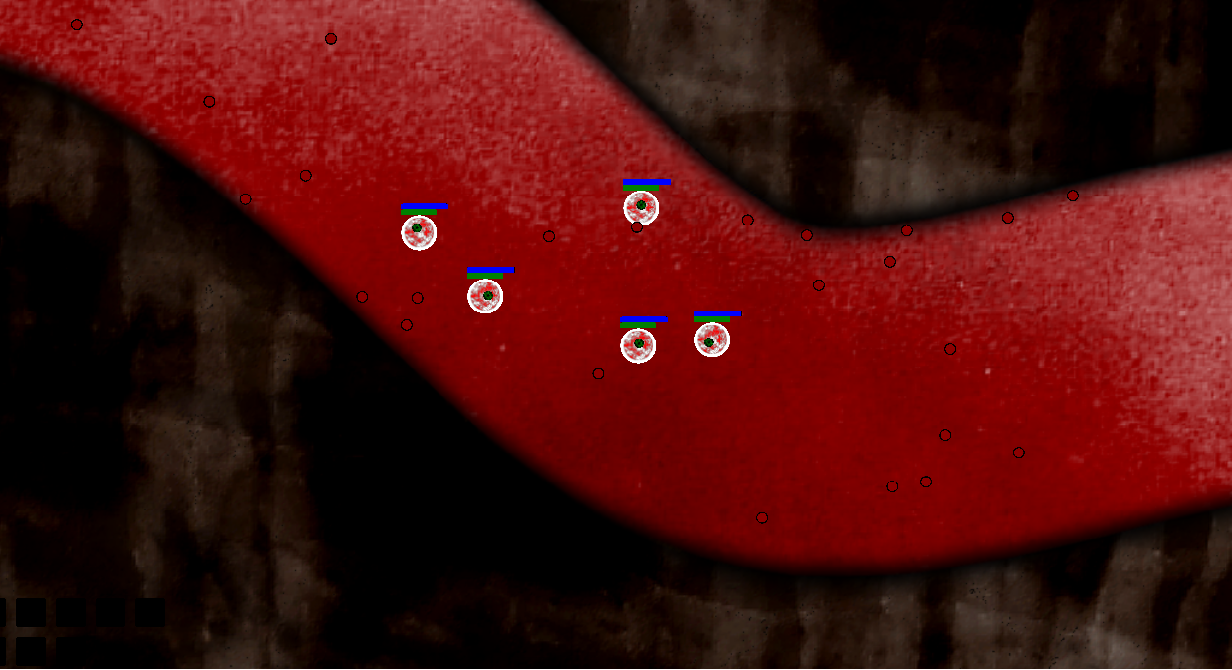
\includegraphics[width=12cm]{img_screenplay/neutral}
  \end{center}
  \caption{Rote Blutkörperchen in einer Blutbahn}
  \label{fig:heamo_virus}
\end{figure}

\begin{figure}[ht]
  \begin{center}
    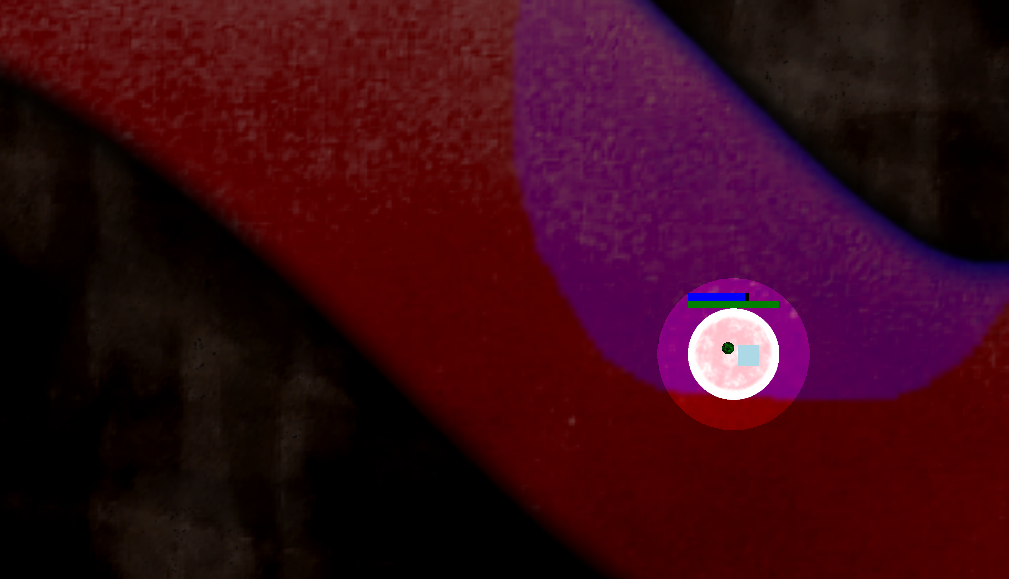
\includegraphics[width=12cm]{img_screenplay/tcell}
  \end{center}
  \caption{T-Zelle im Mutationsfeld}
  \label{fig:tcell}
\end{figure}

\begin{figure}[ht]
  \begin{center}
    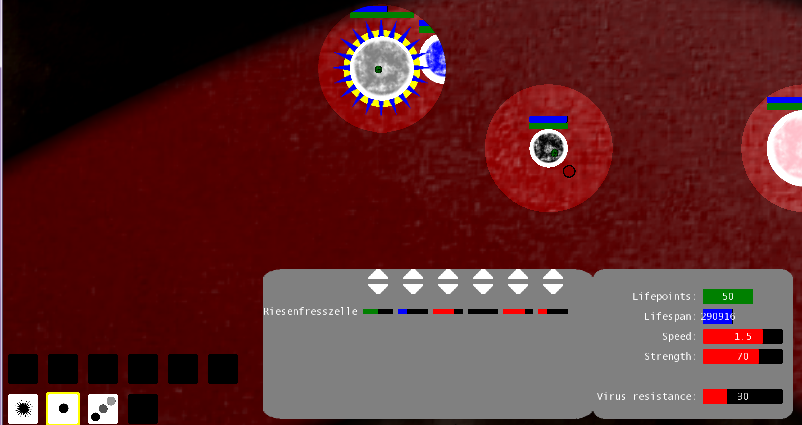
\includegraphics[width=12cm]{img_screenplay/riesenfresszelle}
  \end{center}
  \caption{Riesenfresszelle (grau), mit Sichtradius, die Virus (blau) angreift.
  Prototyp des HUD.}
  \label{fig:macrophage}
\end{figure}


%Konzeptzeichnungen & Storyboards
%Bilder sind wichtig für den ersten Eindruck. Vor allem im GDD sind Konzeptzeichnungen und Skizzen gut aufgehoben. Auf diese Weise kann man nicht nur sich selbst schnell eine Vorstellung von den Ideen machen, sondern auch anderen vermitteln, worum es im Spiel geht und wie das Spiel und seine Geschichte aussieht. 


\end{document}
